\textbf{{局部性原理:}}通过大量典型程序的分析,发现CPU从主存取指令或取数据,在一定时间内,只是对主存局部地址区域的访问(如循环程序、一些常数)。于是人们就想到一个办法,将CPU近期需要的程序提前存放到Cache中。这样CPU只需访问Cache就可以得到所需要的数据了。一般Cache采用高速的SRAM制作(主存一般使用DRAM),其价格比主存高,容量远比主存小。

\textbf{{主存和Cache的编址}}

下图为Cache-主存存储空间的基本结构。

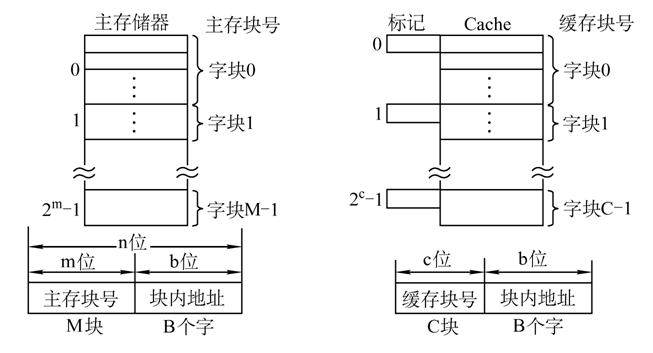
\includegraphics[width=3.46875in,height=1.87500in]{png-jpeg-pics/DE7334A86E795B5566B1263B7DE9D037.png}

\textbf{(1)主存}

从上图中可以看出,主存由一个个的字块组成,当然每个字块包含N个字。主存的地址应该分为两部分:{一部分用来寻找某个字块;另一部分用来寻找该字块中的字或字节}(至于是字还是字节,需要看是哪种寻址方式,在后面例题中会详细讲解)。从上图中可以看出,主存的地址被分为两部分:高m位表示主存的块地址,低b位表示其块内的字或字节数,则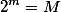
\includegraphics[width=0.63542in,height=0.12500in]{texmath/71ef852mM}表示主存的总块数。

\textbf{(2)Cache}\\
同样,Cache的地址也应该分为两部分:高c位表示Cache的块号,低b位表示其块内的字或字节数,则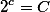
\includegraphics[width=0.52083in,height=0.12500in]{texmath/69348f2cC}表示Cache的总块数,当然Cache的块数C应当远远小于主存块数M。

\textbf{既然C远远小于主存块数M,}一个缓存块不能唯一地、永久地对应一个主存块(因此在上图中给Cache设置了标记,相当于主存块的编号),那么肯定会存在一种情况,即某时刻CPU要访问的信息不在Cache中了,那应该怎么办?这种情况称为Cache不命中,或者Cache缺失。通常使用``命中率''或者``缺失率''来衡量Cache的效率。

\textbf{{Cache的基本结构}}

讲解之前需要分析一下,Cache的基本结构应该由哪几大部分组成?首先,CPU送来的主存地址怎么能转换成Cache地址?这需要一个地址映射变换机构(手动滑一下,参考后面的知识点讲解)。其次,如果Cache内容已满,无法接受来自主存的块时,怎么去给Cache腾出位置来?这需要一个替换机构{(手动滑一下,参考后面的知识点讲解),见下图}。

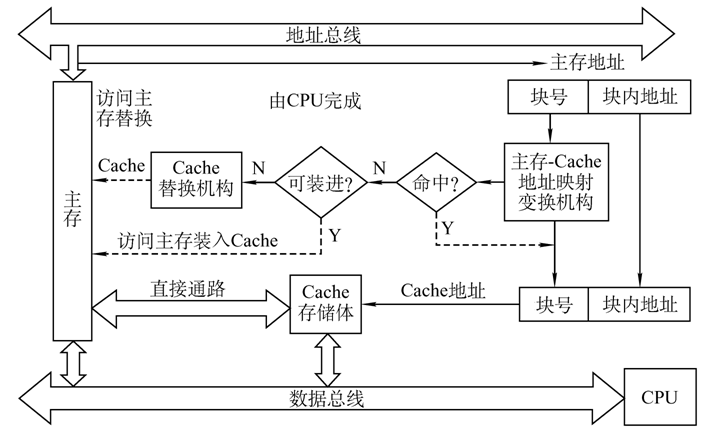
\includegraphics[width=3.69792in,height=2.27083in]{png-jpeg-pics/DE4E63B93B4FDC207CE889BDCC0EAD7A.png}
